This section will elaborate on the steps we took to verify the results in the paper. The following steps were taken:

\begin{itemize}
	\item Generate graphs similar to the ones used in the paper.
	\item Implement the proposed algorithms to create optimized SQL queries from the graphs.
	\item Send query to SQL engine and measure the execution time
\end{itemize}

\noindent Figure~\ref{fig:process} gives an overview of the process and how the results are passed. The generation and translation of graphs are implemented in Java. The idea is to have a graph generator, which outputs the graph we want to solve. Specifically, we pass a list of graphs, which will be the graphs used for a single experiment, varying in graph order or density. \\

The graph translation part takes the graphs as input and generates SQL queries for the graphs, according to the algorithms proposed in the paper. This part thus returns several SQL queries, in a text-file and can be passed directly to the next part in the process. This is the biggest part of the assignment, so we want worked in parallel on the different algorithms. \\

The queries are passed to a SQL engine. We have chosen to use PostgreSQL, to stay close to the tools that were used in the paper. However, we no longer have access to the older version of Postgres that is used by the authors of the paper, so we choose to use a newer version, namely 9.3.4. The newer version can be more optimized, so we have to take this into account when comparing results. Furthermore, we know that the authors used a Linux cluster of Itanium II, processors with 4GB of memory. We have no access to the cluster and no further details about the hardware are available, so we have to use our own machines. The machine we will use has 32GB of RAM, but we are unsure whether our set-up, using an Intel Core i5-4670K (3.40 GHz), can match the computational power of the cluster. 

\begin{figure}
	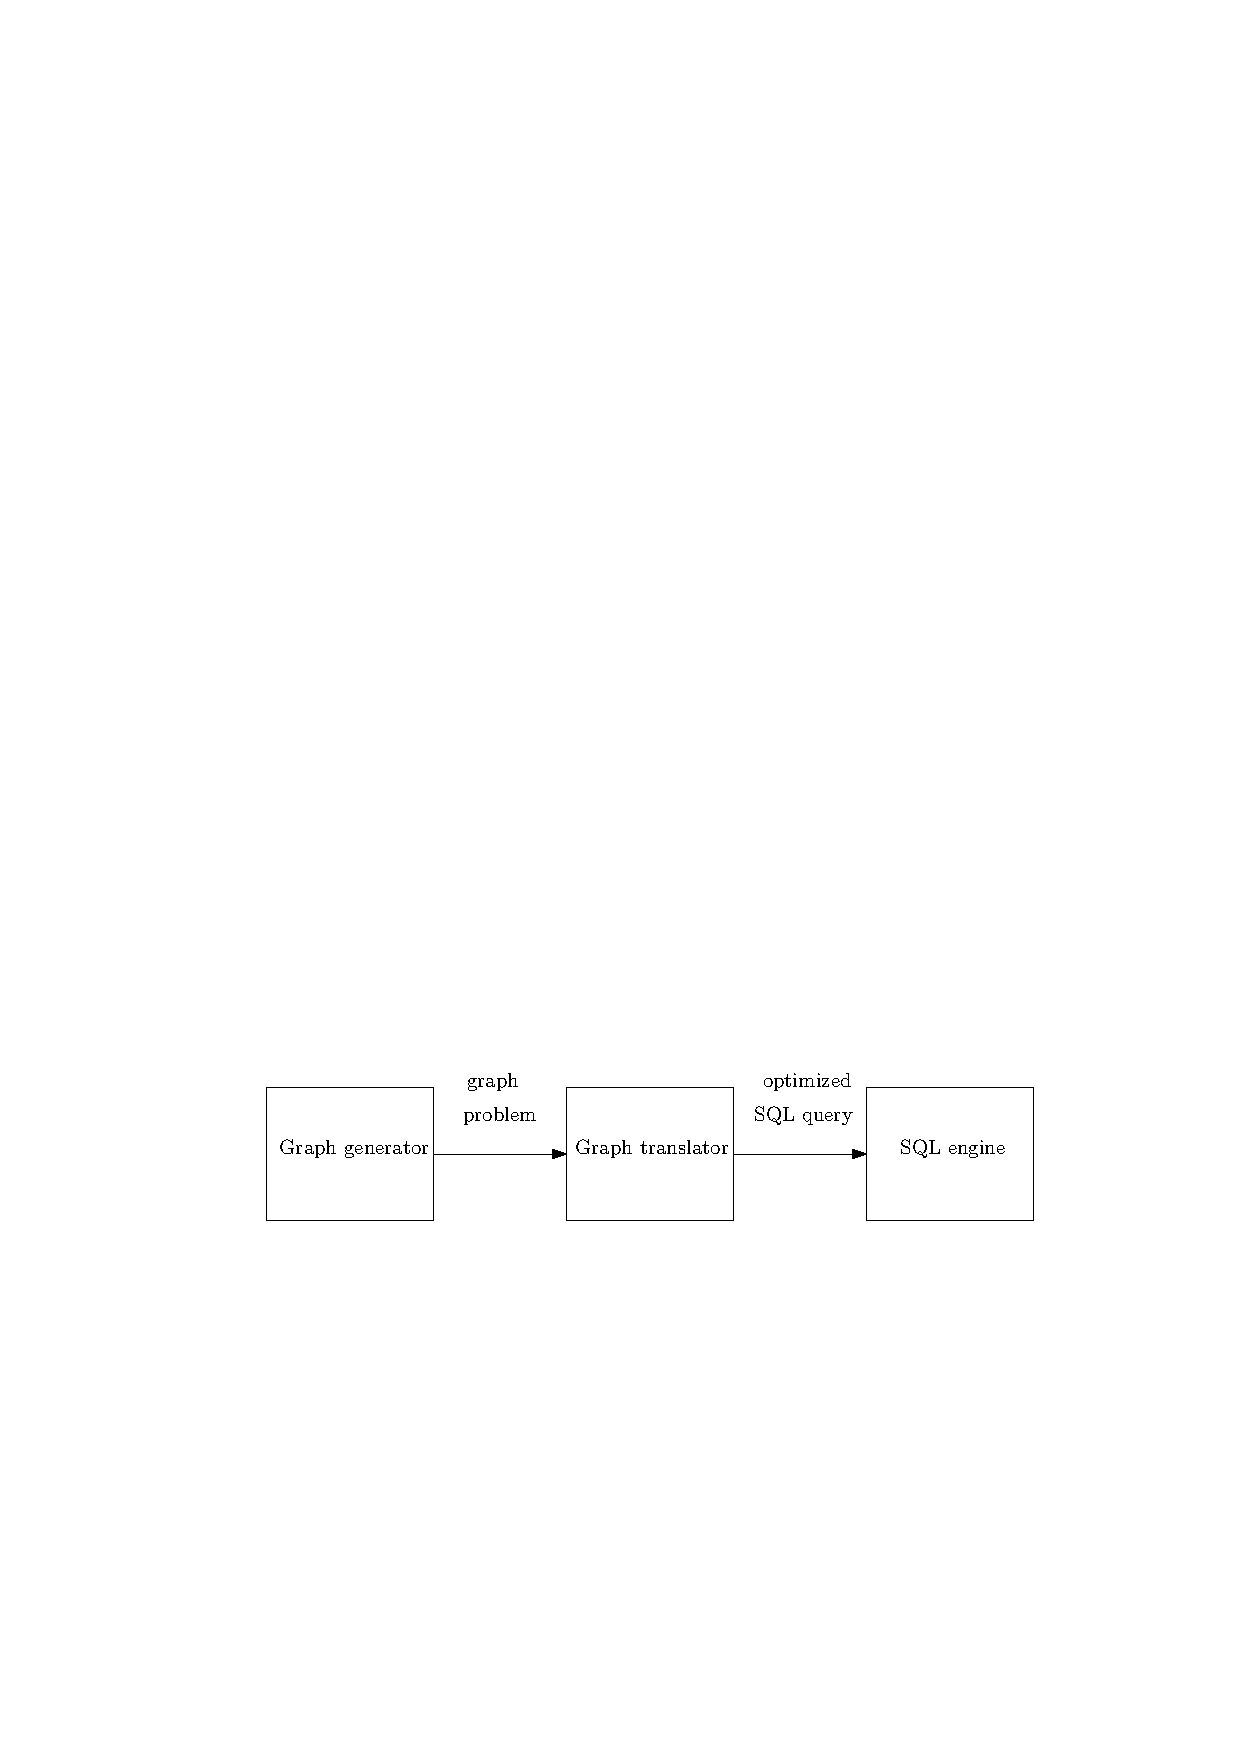
\includegraphics{figures/process.pdf}
	\caption{All steps in the process of verification}
	\label{fig:process}
\end{figure}

\subsection{Bucket Elimination} \label{subsec:MethodologyBucketElim}
Bucket Elimination method represents the query as a join-expression tree which has set of attributes as nodes, in order to describe an evaluation order to the join operation. More specifically, join operations are evaluated from the lower to the higher one and projection operations are applied for this specific evaluation as soon as possible.  The name of this technique is due to the fact that it creates a bucket per variable, which investigates. To clarify how this method works let’s take an order of $n$ query attributes, for which we build $n$ buckets, one per attribute. Inside $bucket_i$ we put all the functions which mention attribute or node $i$. The follow algorithm describes the general idea of the technique.

\begin{enumerate}
\item Process buckets backwards according the given order of nodes.
\item Eliminate the node in the bucket from subsequent computation.
\item Place the computed function from the bucket into the highest variable or node in its scope bucket. \\
Given order: A, C, B, F, D, G \\
Backwards order: G, D, F, B, C, A
\item Eliminate ONE bucket per time (from the $n^{th}$ bucket to the $1^{st}$. 
\end{enumerate}

\paragraph{Preparation for Bucket Elimination Algorithm execution} 
In order to execute the algorithm we have to define an order of nodes as it is mentioned in step 1. Thus we find the MCS order of the vertices. MCS is the acronym of Maximum Cardinality Search and MCS algorithm chooses iteratively vertices. The way in which this algorithm produce the output order is explained as  “the next (unnumbered) vertex to be chosen: the vertex with the most already numbered neighbours”. The follow algorithm describes how the algorithm works.
%TODO fix algo
%\begin{algorithm}
%\begin{algorithmic}
%\Require{Graph $G(V,E)$}
%\Ensure{Ordering $\sigma$ of graph $G$}
%Ordering $\sigma$ of graph G
%\State Assign the label 0 to all vertices.  \Comment{\texttt{each vertex has a label}}
%\For{i \gets 0 \to $n$}
%	\State \text{pick the unnumbered vertex $v$ with the maximum label.}
%	\State \Comment{\texttt{During the first pick, algorithm chooses a random vertex, since all vertices have label equal to 0.}}
%	\State $\sigma(i)$ \gets $v$
%	\ForAll{\text{unnumbered vertex $w$ adjacent to vertex $v$}}
%		\State increment $label(2)$ by 1.
%\EndFor
%\EndFor
%\end{algorithmic}
%\end{algorithm}

\paragraph{Bucket Elimination Algorithm Execution}
Given the MCS order of the vertices we create a bucket for each vertex and now we consider these buckets iteratively, from the last to the first and eliminate the latest bucket every time (bottom up method). The Bucket of the vertex $v_i$ stores:
\begin{itemize}
\item Every edge, which contains vertex $v_i$. $edge(v_i,X) edge(X,v_i)$
\item Every query regarding vertex $v_i$
\end{itemize}
\noindent During these iterations, inside the considering bucket there are several relations, where there is a specific attribute, iconic for this bucket, in all these relations. For all these relations, their join is computed and attributes are projected out, if they do not belong to the target schema, which we want in the end. For this reason, each bucket has live vertices. These are:
\begin{itemize}
\item Every vertex, which appear inside the edges of the bucket. $edge(v_i,LiveVertex) edge(LiveVertex,v_i )$
\item Every vertex, which appear inside SELECT section of bucket’s queries
\end{itemize}
So, as mentioned above, we process these buckets in descending order according to MCS order in the following way. A bucket is processed by this way:

\begin{enumerate}
\item Create the following query \\
\underline{SELECT} all the \emph{live vertices} of the bucket \\
\underline{FROM} all \emph{edges} and \emph{queries} of the bucket\\
\underline{JOINing} them \\
\underline{ON} \emph{straightforward} approach conditions
\item Find the destination of the above query between the live vertices of the bucket. This means that we have to find the maximal vertex in query’s  SELECT section. With the term maximal, we indicate the vertex with the position which is closer to the first one according the MCS order. 
\item Move the query, which is created during the first step, to chosen vertex’s bucket and then eliminate the processed bucket.
\end{enumerate}

When we reach the final bucket we will not execute the $2^{nd}$ and the $3^{rd}$ step, but we will change the SELECT section, with SELECTing only one vertex in Boolean case or SELECTing the free vertices in non-Boolean case.

The result can be empty, and in that case the result of the whole query is empty. If it is not empty, we place the resulting relation in the highest bucket, which has an attribute in the joined relation that is iconic for the bucket. If this process terminates with there still being a relation in the last bucket, we have found the non-empty result of our query.

\subsection{Other approaches} \label{subsec:MethodologyOtherApproaches}
\paragraph{Naive} The naive approach put all edges in the FROM clause and puts all the conditions in the WHERE clause. This means that for each node the value must be the same. This is done by forcing this equality for the nodes on  each edge only on the first edge the node occurred in. 

\paragraph{Straightforward} The straightforward approach uses the same idea, only uses the JOIN operation instead of all the edges in the FROM clause. 

\paragraph{Early Projection and Reordering} The early projection approach tries to project out all nodes that are not occurring in the later part of the computation / query.  It does so by creating a sub-query of the query and uses this sub-query to continue building the query. The reordering approach just changes the order in which the nodes are projected out. 